\begin{figure}[!h]
\centering
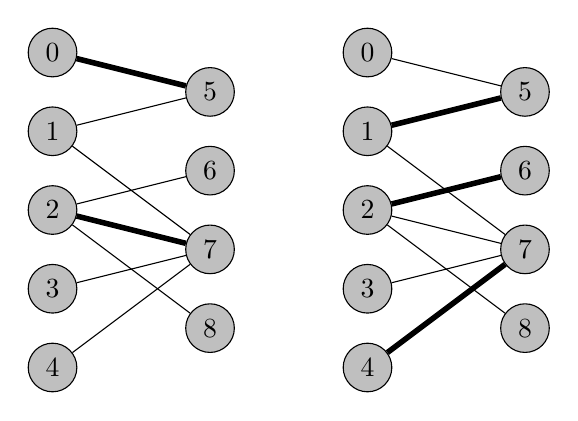
\begin{tikzpicture}[scale=1, vertex/.style = {circle,fill=gray!50,draw}, edge1/.style = {-}, edge2/.style = {-,line width=2pt}]
% vertex
\node[vertex] (n0) at (1,5)  {0};
\node[vertex] (n1) at (1,4)  {1};
\node[vertex] (n2) at (1,3)  {2};
\node[vertex] (n3) at (1,2)  {3};
\node[vertex] (n4) at (1,1)  {4};
\node[vertex] (n5) at (3,4.5)  {5};
\node[vertex] (n6) at (3,3.5)  {6};
\node[vertex] (n7) at (3,2.5)  {7};
\node[vertex] (n8) at (3,1.5)  {8};
%edges
\draw[edge1] (n1) to (n5);
\draw[edge1] (n1) to (n7);
\draw[edge1] (n2) to (n6);
\draw[edge1] (n2) to (n8);
\draw[edge1] (n3) to (n7);
\draw[edge1] (n4) to (n7);
\draw[edge2] (n0) to (n5);
\draw[edge2] (n2) to (n7);
% vertex
\node[vertex] (n10) at (5,5)  {0};
\node[vertex] (n11) at (5,4)  {1};
\node[vertex] (n12) at (5,3)  {2};
\node[vertex] (n13) at (5,2)  {3};
\node[vertex] (n14) at (5,1)  {4};
\node[vertex] (n15) at (7,4.5)  {5};
\node[vertex] (n16) at (7,3.5)  {6};
\node[vertex] (n17) at (7,2.5)  {7};
\node[vertex] (n18) at (7,1.5)  {8};
%edges
\draw[edge1] (n10) to (n15);
\draw[edge1] (n11) to (n17);
\draw[edge1] (n12) to (n17);
\draw[edge1] (n12) to (n18);
\draw[edge1] (n13) to (n17);
\draw[edge2] (n11) to (n15);
\draw[edge2] (n12) to (n16);
\draw[edge2] (n14) to (n17);
\end{tikzpicture}
\caption{Ejemplo de emparejamiento bipartito}
Un grafo bipartito $G=(V,E)$ con partición de vértices $V=L \cup R$. Un emparejamiento con cardinalidad 2, un emparejamiento máximo con cardinalidad 3. \\Fuente: \cite{Cormen2009}.
\label{empBip}
\end{figure}